% v13 --- Problem, Introduction, and the switched model. Owner's plan,
% 2026-09-04:
%   * the PROBLEM is bullet facts 1/2/3 answering "why must it switch", drawn
%     from docs/EECON49_[Nui](1).md section 1;
%   * the INTRODUCTION page carries Figure 1 from docs/source/figures plus the
%     m_i equation;
%   * the NEXT page carries Figure 2 plus the state vectors X_sys, x_IBR, x_SG,
%     x_GFL, x_GFM;
%   * the cover's title box takes the same colour as the top and bottom bars.
% Nothing else yet -- this is v13's whole scope.
%
% FIGURE NUMBERING follows the source paper's own, which is why Figure 1 is the
% electrical model and Figure 2 the control structure: the red dashed box inside
% Figure 1 points at "รูปที่ 2", and with this order that pointer still lands on
% the right page.
%
% COVER COLOUR. Measured from the v12 render: the frametitle bar is
% myblue!82!black = RGB(0,0,146), the footline was Berlin's own RGB(38,38,134),
% and the cover box was RGB(51,51,178) -- three different blues. All three are
% now myblue!82!black, so "same as the top and bottom bars" is true of the bars
% themselves as well, not just of the cover.
\documentclass{beamer}
\usepackage{fontspec}
\setsansfont[Path=C:/Users/User/AppData/Local/Microsoft/Windows/Fonts/,UprightFont=Helvetica.ttf,BoldFont=Helvetica-Bold.ttf,ItalicFont=Helvetica-Oblique.ttf,BoldItalicFont=Helvetica-BoldOblique.ttf]{Helvetica.ttf}
\usetheme{Berlin}
\usefonttheme[onlymath]{serif}
\usepackage{xcolor}
\usepackage{graphicx}
\usepackage{amsmath,amsfonts,amssymb}
\usepackage{bm}
\setcounter{MaxMatrixCols}{20}
\usepackage{booktabs,array,multicol}
\usepackage{tikz}
\usetikzlibrary{arrows.meta,positioning,shapes}

\definecolor{myblue}{rgb}{0.0,0.0,0.7}
\definecolor{pnavy}{HTML}{0F2A4A}
\definecolor{pblue}{HTML}{1D5288}
\definecolor{pgreen}{HTML}{1E7E34}
\definecolor{pred}{HTML}{A93226}
\definecolor{pyellow}{HTML}{B7950B}
% The one bar colour, used by the frametitle, the footline and the cover box.
\colorlet{barblue}{myblue!82!black}

\setbeamercolor{item}{fg=myblue}
\setbeamercolor{block title}{bg=barblue,fg=white}
\setbeamercolor{block body}{bg=blue!7,fg=black}
\setbeamercolor{itemize item}{fg=myblue}
\setbeamertemplate{navigation symbols}{}
\setbeamercolor{frametitle}{bg=barblue,fg=white}
\setbeamertemplate{section in toc}[sections numbered]
\setbeamertemplate{background}{}
\setbeamertemplate{headline}{}
% Numbered figures and equations, per the standing rule: every figure and every
% equation must carry a number so it can be pointed at during questions.
%
% CAPTIONS ARE CENTRED AND SAY WHAT THE FIGURE IS, nothing more (owner, 2026-09-05):
% Beamer's default caption template is a flush-left paragraph, which on a one-line
% caption reads as a stray sentence under the artwork. This template centres it and
% keeps the numbered label inline. Findings belong in the talk, not under the picture.
\setbeamertemplate{caption}[numbered]
\setbeamertemplate{caption}{\centering\insertcaptionname~\insertcaptionnumber:
  \insertcaption\par}
\setbeamerfont{caption}{size=\scriptsize}
\setbeamercolor{caption name}{fg=barblue}
% Berlin's footline draws its own two colour boxes in author/date colours. Both
% are set to barblue so the strip matches the frametitle exactly.
\setbeamercolor{author in head/foot}{bg=barblue,fg=white}
\setbeamercolor{date in head/foot}{bg=barblue,fg=white}
\setbeamertemplate{footline}{%
  \leavevmode%
  \hbox{%
  \begin{beamercolorbox}[wd=.88\paperwidth,ht=2.6ex,dp=1.1ex,leftskip=1.2em]{author in head/foot}%
    \ifodd\insertframenumber\relax
      \scriptsize An Automatic Following/Forming Framework for Inverter-Based Resources%
    \else
      \scriptsize Department of Electrical Engineering, School of Engineering, KMITL%
    \fi
  \end{beamercolorbox}%
  \begin{beamercolorbox}[wd=.12\paperwidth,ht=2.6ex,dp=1.1ex,center]{date in head/foot}%
    \scriptsize \insertframenumber/\inserttotalframenumber
  \end{beamercolorbox}}%
}

\newcommand{\pu}{\,\mathrm{p.u.}}

% The two status marks of the summary page. Drawn in tikz rather than set from a
% symbol font: fontspec loads Helvetica for text, which carries neither a tick nor a
% ballot box, and amssymb's \checkmark would arrive in a different typeface from every
% other glyph on the slide. baseline pulls the box onto the text baseline so a row of
% the table does not sit low.
\newcommand{\ckbox}{\tikz[baseline=-0.055cm]{%
  \draw[line width=0.6pt,pgreen] (0,0) rectangle (0.26,0.26);
  \draw[line width=1.0pt,pgreen] (0.055,0.145) -- (0.115,0.062) -- (0.215,0.205);}}
\newcommand{\opbox}{\tikz[baseline=-0.055cm]{%
  \draw[line width=0.6pt,black!55] (0,0) rectangle (0.26,0.26);}}

\begin{document}

% ========================= 1. COVER =====================================
% The title box is barblue, the same colour as the frametitle and footline bars.
\begin{frame}[plain]
\centering
\vspace{0.75cm}
\begin{beamercolorbox}[wd=0.86\paperwidth,sep=0.22cm,center]{frametitle}
{\Large\bfseries An Automatic Following/Forming Framework\\for Inverter-Based Resources}
\end{beamercolorbox}
\vspace{0.60cm}
{\fontsize{10.5}{13}\selectfont
Phichitchai Jueajan\quad 66010569\\
Pakkapol Phdungdan\quad 66010612\\[0.20cm]
Advisor: Dr. Tossaporn Surinkaew\\
Co-advisor: Prof. Dr. Issarachai Ngamroo\\[0.45cm]
Department of Electrical Engineering, School of Engineering\\
King Mongkut's Institute of Technology Ladkrabang (KMITL)
}
\end{frame}

% v15: เนื้อหาจาก PW-6916 และ MATLAB; หน้าปกคงเดิม
\setlength{\abovedisplayskip}{5pt}
\setlength{\belowdisplayskip}{5pt}
\begin{frame}{Table of Contents}
\vspace{2mm}
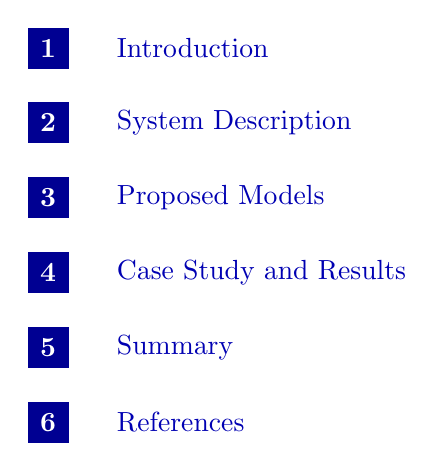
\begin{tikzpicture}[font=\normalsize]
\node[fill=barblue,text=white,minimum size=.52cm,inner sep=1pt,font=\bfseries] at (0,0) {1};
\node[anchor=west,text=myblue] at (.75,0) {Introduction};
\node[fill=barblue,text=white,minimum size=.52cm,inner sep=1pt,font=\bfseries] at (0,-.95) {2};
\node[anchor=west,text=myblue] at (.75,-.95) {System Description};
\node[fill=barblue,text=white,minimum size=.52cm,inner sep=1pt,font=\bfseries] at (0,-1.90) {3};
\node[anchor=west,text=myblue] at (.75,-1.90) {Proposed Models};
\node[fill=barblue,text=white,minimum size=.52cm,inner sep=1pt,font=\bfseries] at (0,-2.85) {4};
\node[anchor=west,text=myblue] at (.75,-2.85) {Case Study and Results};
\node[fill=barblue,text=white,minimum size=.52cm,inner sep=1pt,font=\bfseries] at (0,-3.80) {5};
\node[anchor=west,text=myblue] at (.75,-3.80) {Summary};
\node[fill=barblue,text=white,minimum size=.52cm,inner sep=1pt,font=\bfseries] at (0,-4.75) {6};
\node[anchor=west,text=myblue] at (.75,-4.75) {References};
\end{tikzpicture}
\end{frame}
\section{Introduction}
\begin{frame}{Nomenclature}
\fontsize{6.2}{7.2}\selectfont
\renewcommand{\arraystretch}{1.0}\setlength{\tabcolsep}{3pt}
\textbf{Symbols}\par\smallskip
\begin{columns}[t,onlytextwidth]
\column{.49\textwidth}
\begin{tabular}{@{}p{1.55cm}>{\raggedright\arraybackslash}p{3.35cm}@{}}
$D_v,M$ & VSG damping / virtual inertia constant\\
$E$ & GFM internal voltage magnitude reference\\
$E'_q,E'_d$ & SG transient internal EMFs ($q$/$d$-axis)\\
$E''_q,E''_d$ & SG subtransient internal EMFs ($q$/$d$-axis)\\
$F_0,F_1$ & IBR vector fields, GFL / GFM branch\\
$f_0,f_{coi},\omega_b$ & nominal / centre-of-inertia frequency; $\omega_b=2\pi f_0$\\
$g=0$ & network current balance at every bus, PF and TS\\
$I_{dc},V_{dc}$ & converter DC-link current / voltage\\
$i_d,i_q$ & converter filter currents ($d$/$q$-axis)\\
$k_p,k_i$ & PI proportional / integral gains\\
$m_i$ & IBR $i$ mode: 0 = GFL, 1 = GFM\\
$P_j,Q_j$ & net active / reactive injection at bus $j$\\
$t$ & time\\
\end{tabular}
\column{.49\textwidth}
\begin{tabular}{@{}p{1.55cm}>{\raggedright\arraybackslash}p{3.35cm}@{}}
$u$ & exogenous inputs: set-points, loads, events\\
$V_i,\theta_i$ & bus $i$ voltage magnitude / phase angle\\
$x$ & full differential state vector\\
$x_{SG},x_{IBR}$ & SG / IBR state vectors\\
$Y$ & network admittance matrix\\
$y$ & algebraic variables: bus voltages\\
$\delta,\omega$ & SG rotor angle / speed\\
$\theta_{PLL},\xi_{PLL}$ & PLL estimated angle / integrator state\\
$\theta_{VSG},\omega_{VSG}$ & VSG internal angle / angular speed\\
$\xi_P,\xi_Q$ & power-loop integrator states\\
$\xi_{Id}^{b},\xi_{Iq}^{b}$ & current-loop integrators, $b\in\{GFL,GFM\}$\\
$\xi_{Vd},\xi_{Vq}$ & voltage-loop integrator states\\
\end{tabular}
\end{columns}\par\smallskip
\textbf{Abbreviations}\par\smallskip
\begin{columns}[t,onlytextwidth]
\column{.49\textwidth}
\begin{tabular}{@{}p{1.55cm}>{\raggedright\arraybackslash}p{3.35cm}@{}}
EMF & electromotive force\\
GFL / GFM & grid-following / grid-forming control\\
IBR & inverter-based resource\\
PF / TS & power flow / time-domain simulation\\
PLL & phase-locked loop\\
SG & synchronous generator\\
VSG & virtual synchronous generator\\
\end{tabular}
\column{.49\textwidth}
\mbox{}
\end{columns}
\end{frame}
\begin{frame}{Introduction}
\begin{columns}[c,onlytextwidth]
\column{.48\textwidth}
\small
\begin{itemize}\setlength{\itemsep}{.30cm}
\item Increasing inverter-based resource (IBR) penetration.
\item Less synchronous-machine inertia.
\item Weak grids challenge PLL-based grid-following (GFL) control.
\item Grid-forming (GFM) control provides voltage and frequency support.
\item Adapt the control mode to grid conditions [1],[2].
\end{itemize}
\column{.48\textwidth}
\centering
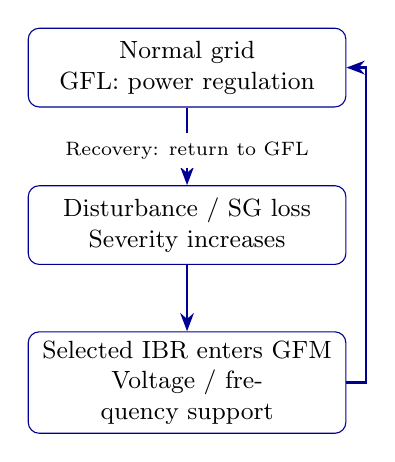
\begin{tikzpicture}[font=\small,b/.style={draw=barblue,rounded corners,align=center,text width=3.8cm,minimum height=1.0cm},a/.style={-{Stealth},thick,barblue}]
\node[b] (a) at (0,2.7) {Normal grid\\GFL: power regulation};
\node[b] (b) at (0,.7) {Disturbance / SG loss\\Severity increases};
\node[b] (c) at (0,-1.3) {Selected IBR enters GFM\\Voltage / frequency support};
\draw[a] (a)--(b);\draw[a] (b)--(c);
\draw[a] (c.east)--++(.25,0)|-(a.east);\node[font=\scriptsize,fill=white] at (0,1.65) {Recovery: return to GFL};
\end{tikzpicture}
\end{columns}
\end{frame}

\section{System Description and Operating Principles}
\begin{frame}{System Description and Operating Principles}
\footnotesize
\begin{columns}[t,onlytextwidth]
\column{.48\textwidth}
\textbf{Power flow}\par
Rotor and converter states are constant; bus currents balance.\par
\begin{equation}
0=g(x,y,u_0,m).
\end{equation}
{\scriptsize
\begin{align}
P^{inj}_i-P_j(x,y,u_0,m)&=0,\\
Q^{inj}_i-Q_j(x,y,u_0,m)&=0.
\end{align}}
\column{.48\textwidth}
\textbf{Time-domain simulation}\par
Machine and converter states respond to disturbances.\par
\begin{align}
\dot x&=f(x,y,u,m,t),\\
0&=g(x,y,u,m,t),\\
m_i&=\begin{cases}0&\text{GFL},\\1&\text{GFM}.\end{cases}
\end{align}
\begin{align}
x&=[x_{SG}^{T},x_{IBR,1}^{T},\ldots,x_{IBR,4}^{T}]^T,\\
x_{SG}&=[\delta,\omega,E_q',E_d',E_q'',E_d'']^T.
\end{align}
\end{columns}
\end{frame}

\section{Proposed Models and Control Structure}
\begin{frame}{IBR Model}
\begin{columns}[c,onlytextwidth]
\column{.48\textwidth}\footnotesize
\textbf{Shared physical states}
\begin{equation}x_p=[i_d,i_q,V_{dc},I_{dc}]^T\end{equation}
\begin{align}
\frac{L_f}{\omega_b}\dot i_d&=v_{cd}-v_d-R_fi_d\notag\\&\quad+\omega_{pu}L_fi_q,\\
\frac{L_f}{\omega_b}\dot i_q&=v_{cq}-v_q-R_fi_q\notag\\&\quad-\omega_{pu}L_fi_d.
\end{align}
\begin{equation}\omega_{pu}=\begin{cases}1+\dot\theta_{PLL}/\omega_b&m_i=0,\\\omega_{VSG}&m_i=1.\end{cases}\end{equation}
\column{.48\textwidth}
\begin{figure}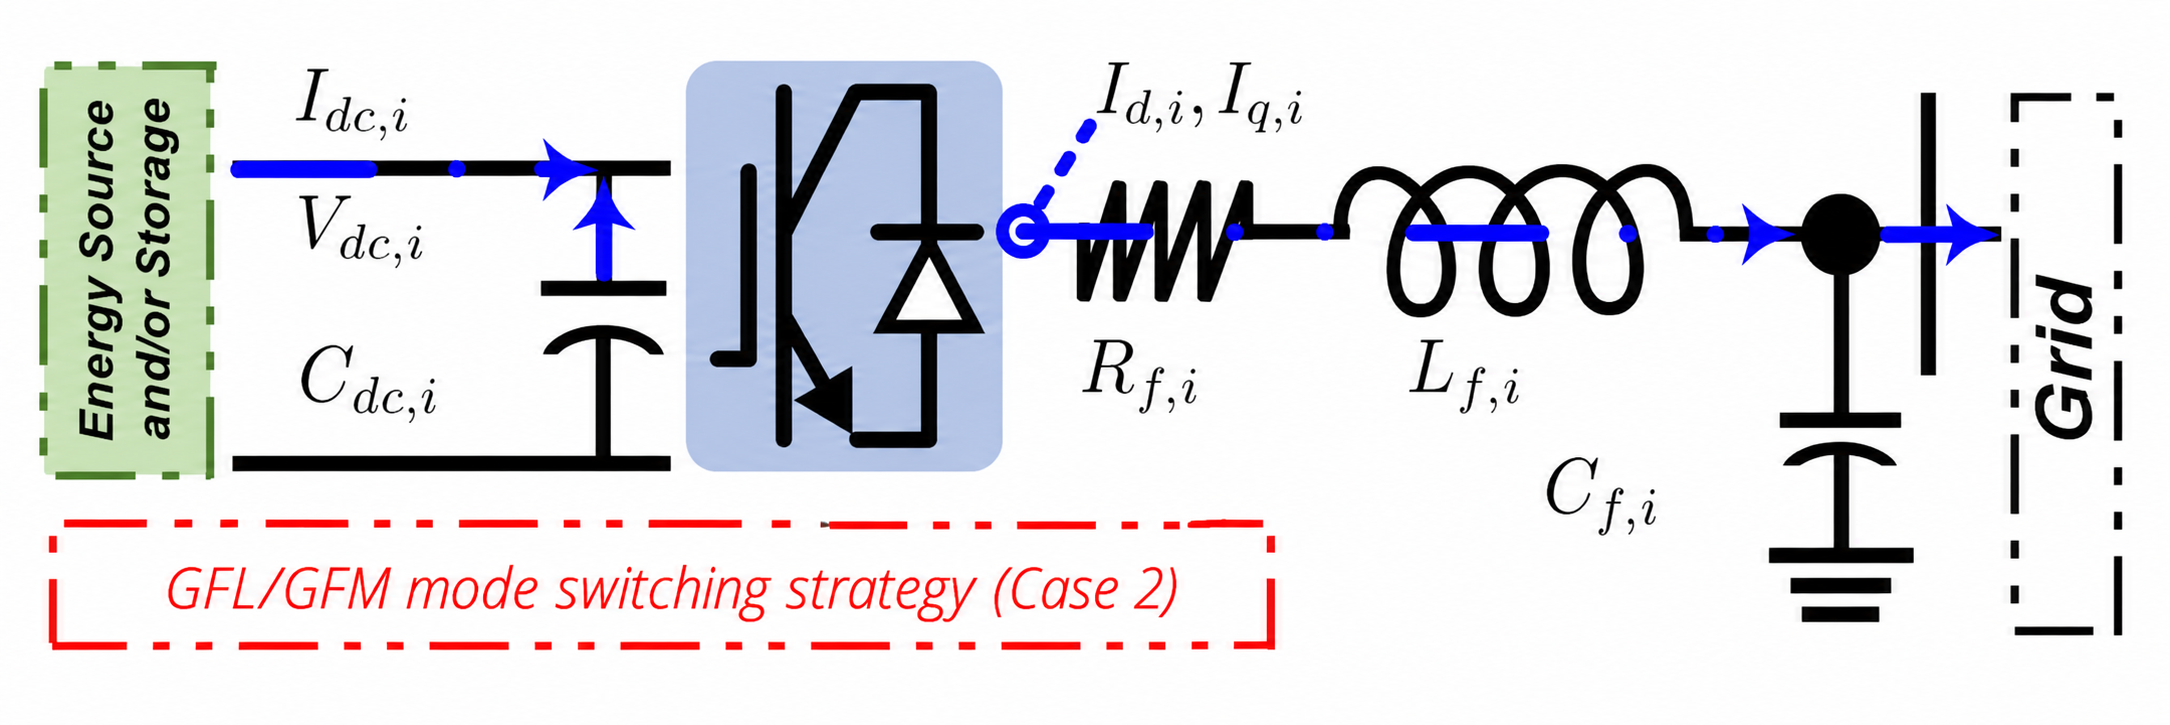
\includegraphics[width=\linewidth]{figures/fig1_ibr_electrical.png}\caption{IBR electrical model.}\label{fig:plant}\end{figure}
{\begin{equation}
\scalebox{0.78}{$
\dot x_{IBR}=\begin{cases}F_0(x_{IBR},y,u)&m_i=0,\\F_1(x_{IBR},y,u)&m_i=1.
\end{cases}$}
\tag*{\scriptsize (13)}
\end{equation}}
\stepcounter{equation}
\end{columns}
\end{frame}

\begin{frame}{Switchable GFL/GFM Control Model}
	\scriptsize
	\begin{columns}[t,onlytextwidth]
		\column{.48\textwidth}
		\raggedright
		\textbf{Controller state vectors}\par
		{\scriptsize
		\setlength{\abovedisplayskip}{3pt}
		\setlength{\belowdisplayskip}{3pt}
		\setlength{\abovedisplayshortskip}{3pt}
		\setlength{\belowdisplayshortskip}{3pt}
		\begin{equation}
			\begin{aligned}
				x_{GFL}=[&\theta_{PLL},\xi_{PLL},\xi_P,\xi_Q,\\[-1pt]
				&\xi_{Id}^{GFL},\xi_{Iq}^{GFL}]^T
			\end{aligned}
		\end{equation}
		\begin{equation}
			\begin{aligned}
				x_{GFM}=[&\theta_{VSG},\omega_{VSG},E,\xi_{Vd},\\[-1pt]
				&\xi_{Vq},\xi_{Id}^{GFM},\xi_{Iq}^{GFM}]^T
			\end{aligned}
		\end{equation}
		}
		\textbf{GFL: PLL + power control}\par
		{\scriptsize
		\setlength{\abovedisplayskip}{3pt}
		\setlength{\belowdisplayskip}{3pt}
		\setlength{\abovedisplayshortskip}{3pt}
		\setlength{\belowdisplayshortskip}{3pt}
		\begin{equation}
			\dot\theta_{PLL}=k_{p,PLL}v_q+k_{i,PLL}\xi_{PLL}
		\end{equation}
		}
		\smallskip
		\textbf{GFM: VSG + voltage control}\par
		{\scriptsize
		\setlength{\abovedisplayskip}{3pt}
		\setlength{\belowdisplayskip}{3pt}
		\setlength{\abovedisplayshortskip}{3pt}
		\setlength{\belowdisplayshortskip}{3pt}
		\begin{equation}
			\begin{aligned}
				M\dot\omega_{VSG}&=\kappa P_{ref}-P_{inv}\\[-1pt]
				&\quad-D_v(\omega_{VSG}-1)
			\end{aligned}
		\end{equation}
		\begin{equation}
			\kappa=S_{base}/M_{base}
		\end{equation}
		\begin{equation}
			\begin{aligned}
				x_{IBR}=[&i_d,i_q,V_{dc},\\[-1pt]
				&x_{GFL}^{T},x_{GFM}^{T},I_{dc}]^T
			\end{aligned}
		\end{equation}
		}
		\column{.50\textwidth}
		\centering
		\vspace{.1cm}
		\begin{figure}
			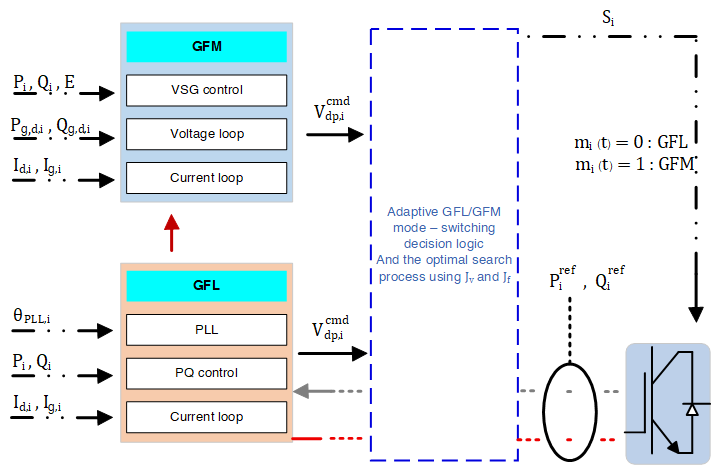
\includegraphics[width=\linewidth,height=6.4cm,keepaspectratio]{figures/intro222222222.png}
			\caption{Switchable controller branches.}
			\label{fig:control15}
		\end{figure}
	\end{columns}
\end{frame}

\begin{frame}{Mode Switching: Supervisory Readiness}
\centering
\begin{figure}
\vspace{2mm}
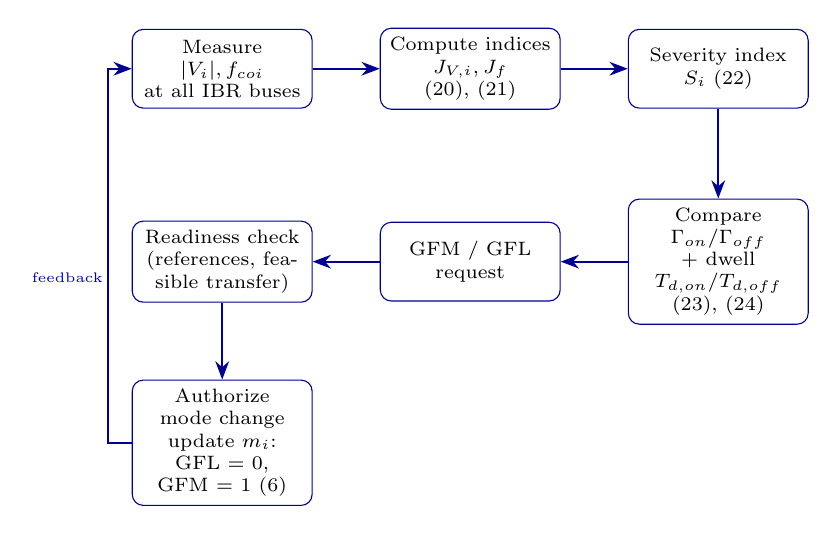
\begin{tikzpicture}[font=\scriptsize,b/.style={draw=barblue,rounded corners,align=center,text width=2.05cm,minimum height=1.0cm},a/.style={-{Stealth},thick,barblue},lbl/.style={font=\tiny,text=myblue,align=center,inner sep=1.5pt}]
\node[b] (v) at (0,0) {Measure $|V_i|,f_{coi}$\\at all IBR buses};
\node[b] (j) at (3.15,0) {Compute indices\\$J_{V,i},J_f$ (20), (21)};
\node[b] (s) at (6.30,0) {Severity index\\$S_i$ (22)};
\node[b] (h) at (6.30,-2.45) {Compare $\Gamma_{on}/\Gamma_{off}$ + dwell $T_{d,on}/T_{d,off}$ (23), (24)};
\node[b] (q) at (3.15,-2.45) {GFM / GFL\\request};
\node[b] (r) at (0,-2.45) {Readiness check\\(references, feasible transfer)};
\node[b] (m) at (0,-4.75) {Authorize mode change\\update $m_i$: GFL = 0, GFM = 1 (6)};
\draw[a](v.east)--(j.west);
\draw[a](j.east)--(s.west);
\draw[a](s.south)--(h.north);
\draw[a](h.west)--(q.east);
\draw[a](q.west)--(r.east);
\draw[a](r.south)--(m.north);
\draw[a](m.west)--++(-0.30,0)|-(v.west) node[lbl,pos=0.22,left]{feedback};
\end{tikzpicture}
\caption{Supervisory readiness and GFL/GFM mode-switching procedure.}
\end{figure}
\end{frame}

\begin{frame}{Mode Switching: Index and Logic}
\footnotesize
\textbf{Voltage and frequency indices}\par
\begin{align}
J_{V,i}&=\frac{\bigl||V_i|-V_i^\star\bigr|}{\Delta V_{base}},\\
J_f&=\frac{|f_{coi}-f_0|}{\Delta f_{base}},\\
S_i&=\operatorname{sat}_{[0,1]}(w_VJ_{V,i}+w_fJ_f).
\end{align}
\medskip{\scriptsize $J_{V,i},J_f$: voltage / centre-of-inertia indices; $S_i\in[0,1]$: severity; $V_i^\star$: healthy per-bus PF magnitude; $\Gamma_{on},\Gamma_{off}$: thresholds; $T_{d,on},T_{d,off}$: dwells; $w_V,w_f$: weights; $\mathcal L,\mathcal G$: online GFL/GFM sets.\par}
\begin{equation}
\text{GFM request:}\quad\exists i\in\mathcal L:\ S_i\ge\Gamma_{on}\quad\text{for }T_{d,on}
\end{equation}
\begin{equation}
\text{GFL request:}\quad\forall i\in\mathcal L\cup\mathcal G:\ S_i<\Gamma_{off}\quad\text{for }T_{d,off}
\end{equation}
\medskip
$\Gamma_{on}/\Gamma_{off}$: 0.65/0.35; dwell: 0.10/1.00 s.\par
Index bases: 0.10 pu, 0.50 Hz; voltage/frequency weights: 0.5/0.5.\par
\end{frame}

\section{Case Study and Simulation Results}
\begin{frame}{Case Study: IEEE 14-Bus System}
\begin{columns}[c,onlytextwidth]
\column{.72\textwidth}\begin{figure}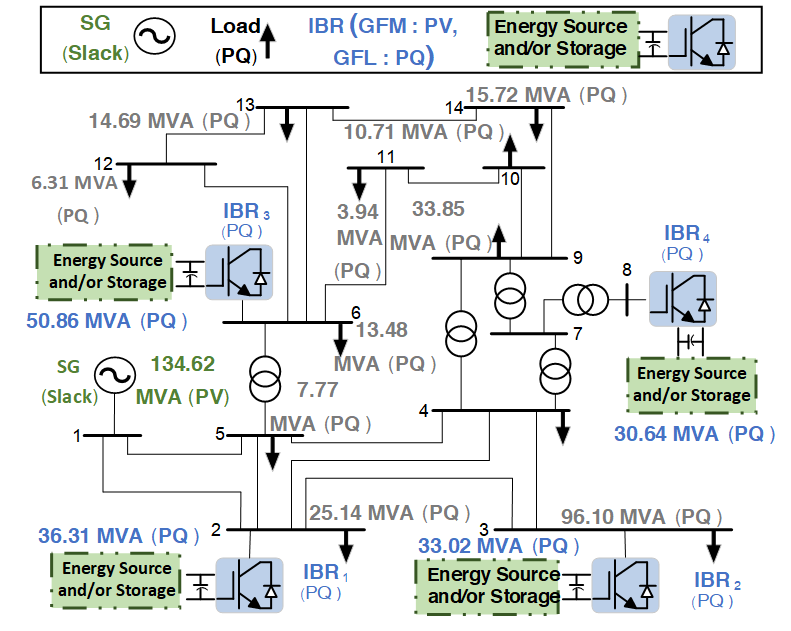
\includegraphics[width=\linewidth,height=6.25cm,keepaspectratio]{figures/fig4_ieee14_network.png}\caption{IEEE 14-bus study network [3].}\end{figure}
\column{.25\textwidth}\small
SG1: Bus 1\\[.25cm]
IBR$_1$: Bus 2\\IBR$_2$: Bus 3\\IBR$_3$: Bus 6\\IBR$_4$: Bus 8\\[.45cm]
100 MVA\\60 Hz
\end{columns}
\end{frame}

\begin{frame}{Parameter Settings: Network and Plant}
\scriptsize
\renewcommand{\arraystretch}{1.22}\setlength{\tabcolsep}{4pt}
\centering
\begin{tabular}{@{}p{3.05cm}p{3.0cm}p{2.55cm}p{1.25cm}@{}}
\toprule Parameter & Symbol & Value & Unit\\\midrule
\multicolumn{4}{@{}l}{\textbf{Network and synchronous machine}}\\
System bases &$S_{base},f_0$&100,60&MVA, Hz\\
SG (system base)&$H,D$&2.50,1.00&s, pu\\
SG time constants&$T'_{d0},T''_{d0},T''_{q0}$&7.40,0.03,0.033&s\\
\multicolumn{4}{@{}l}{\textbf{IBR plant}}\\
Filter&$L_f,R_f$&0.15,0.015&pu\\
DC bus / current limit&$C_{dc},V_{dc}^{0},I_{max}$&0.10,1.00,1.20&pu\\
DC source&$\epsilon_{dc},P_r,\tau_s,\zeta^\star$&0.10,1.00,0.005,0.707&--, pu, s, --\\
Chopper&$V_{dc}^{max},\delta_{ch}$&1.10,0.02&pu, --\\
\bottomrule
\end{tabular}\par
\medskip
\raggedright\scriptsize
* Units follow the normalized controller equations.\par

\end{frame}
\begin{frame}{Parameter Settings: Control and Supervisor}
\scriptsize
\renewcommand{\arraystretch}{1.22}\setlength{\tabcolsep}{4pt}
\centering
\begin{tabular}{@{}p{3.05cm}p{3.0cm}p{2.55cm}p{1.25cm}@{}}
\toprule Parameter & Symbol & Value & Unit\\\midrule
\multicolumn{4}{@{}l}{\textbf{GFL control}}\\
PLL PI gains&$k_{p,PLL},k_{i,PLL}$&1.20, 5.00&*\\
Power PI gains&$k_{p,P/Q},k_{i,P/Q}$&0.80, 2.50&*\\
\multicolumn{4}{@{}l}{\textbf{Shared current loop}}\\
Current PI&$k_{p,I},k_{i,I}$&0.30,4.00&*\\
\multicolumn{4}{@{}l}{\textbf{GFM control}}\\
VSG&$M,D_v$&0.08, 20.0&pu$^\dagger$\\
Q--V loop&$k_Q,k_E,\tau_E$&0.25,8.00,0.05&*, *, s\\
Voltage PI&$k_{p,V},k_{i,V}$&1.20, 4.50&*\\
\multicolumn{4}{@{}l}{\textbf{Supervisor}}\\
Hysteresis&$\Gamma_{on},\Gamma_{off}$&0.65,0.35&--\\
Dwell / weights&$T_{d,on/off};w_V,w_f$&0.10/1.00;0.5,.50&s; --\\
Hold / lock&$T_{hold},T_{lock}$&1.000, 2.000&s\\
Index bases&$\Delta V_{base},\Delta f_{base}$&0.10,0.50&pu, Hz\\
\bottomrule
\end{tabular}\par
\medskip
\raggedright\scriptsize
* Units follow the normalized controller equations.\par
$\dagger$ Report notation: $M=2H_v$, $H_v=0.04$ s.\par
\end{frame}

\begin{frame}{Scenario Timeline}
\centering
\begin{figure}
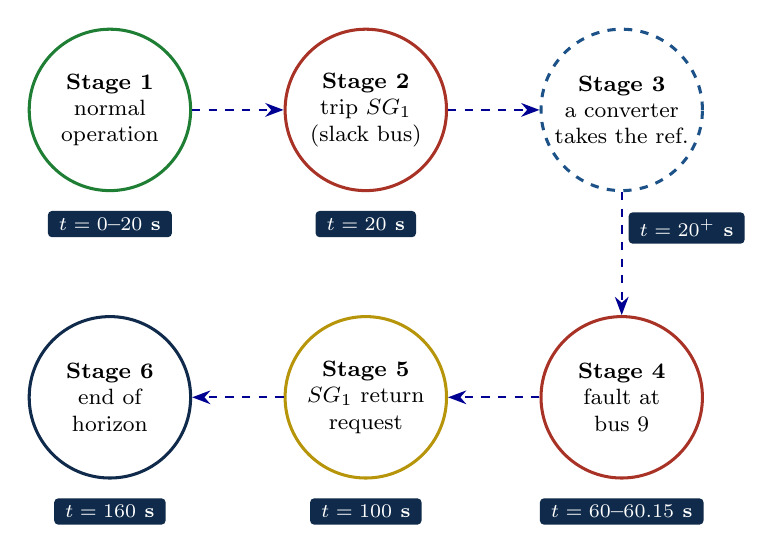
\begin{tikzpicture}[font=\small,xshift=-1.25cm,
  c/.style={circle,draw,line width=1.1pt,align=center,minimum size=2.05cm,inner sep=1pt,font=\footnotesize},
  tag/.style={font=\scriptsize\bfseries,text=white,fill=pnavy,rounded corners=1.5pt,inner xsep=4pt,inner ysep=2.5pt},
  a/.style={-{Stealth},thick,barblue,dashed}]
% --- top row: stages 1 -> 2 -> 3 ---
\node[c,draw=pgreen] (s1) at (0,0) {\textbf{Stage 1}\\normal\\operation};
\node[c,draw=pred] (s2) at (3.25,0) {\textbf{Stage 2}\\trip $SG_1$\\(slack bus)};
\node[c,draw=pblue,dashed] (s3) at (6.50,0) {\textbf{Stage 3}\\a converter\\takes the ref.};
\draw[a] (s1)--(s2);\draw[a] (s2)--(s3);
\node[tag] at (0,-1.45) {$t=0$--$20$ s};
\node[tag] at (3.25,-1.45) {$t=20$ s};
\node[tag,anchor=west] at (6.58,-1.5) {$t=20^{+}$ s};
% --- bottom row: stages 4 -> 5 -> 6 (right to left) ---
\node[c,draw=pred] (s4) at (6.50,-3.65) {\textbf{Stage 4}\\fault at\\bus 9};
\node[c,draw=pyellow] (s5) at (3.25,-3.65) {\textbf{Stage 5}\\$SG_1$ return\\request};
\node[c,draw=pnavy] (s6) at (0,-3.65) {\textbf{Stage 6}\\end of\\horizon};
\draw[a] (s3)--(s4);\draw[a] (s4)--(s5);\draw[a] (s5)--(s6);
\node[tag] at (6.50,-5.10) {$t=60$--$60.15$ s};
\node[tag] at (3.25,-5.10) {$t=100$ s};
\node[tag] at (0,-5.10) {$t=160$ s};
\end{tikzpicture}
\caption{Scenario timeline. Breaker reclose after synchronism: $102.363$ s; final IBR return to GFL: $116.238$ s.}
\end{figure}
\end{frame}

\begin{frame}{Result: IBR State Response}
\centering\begin{figure}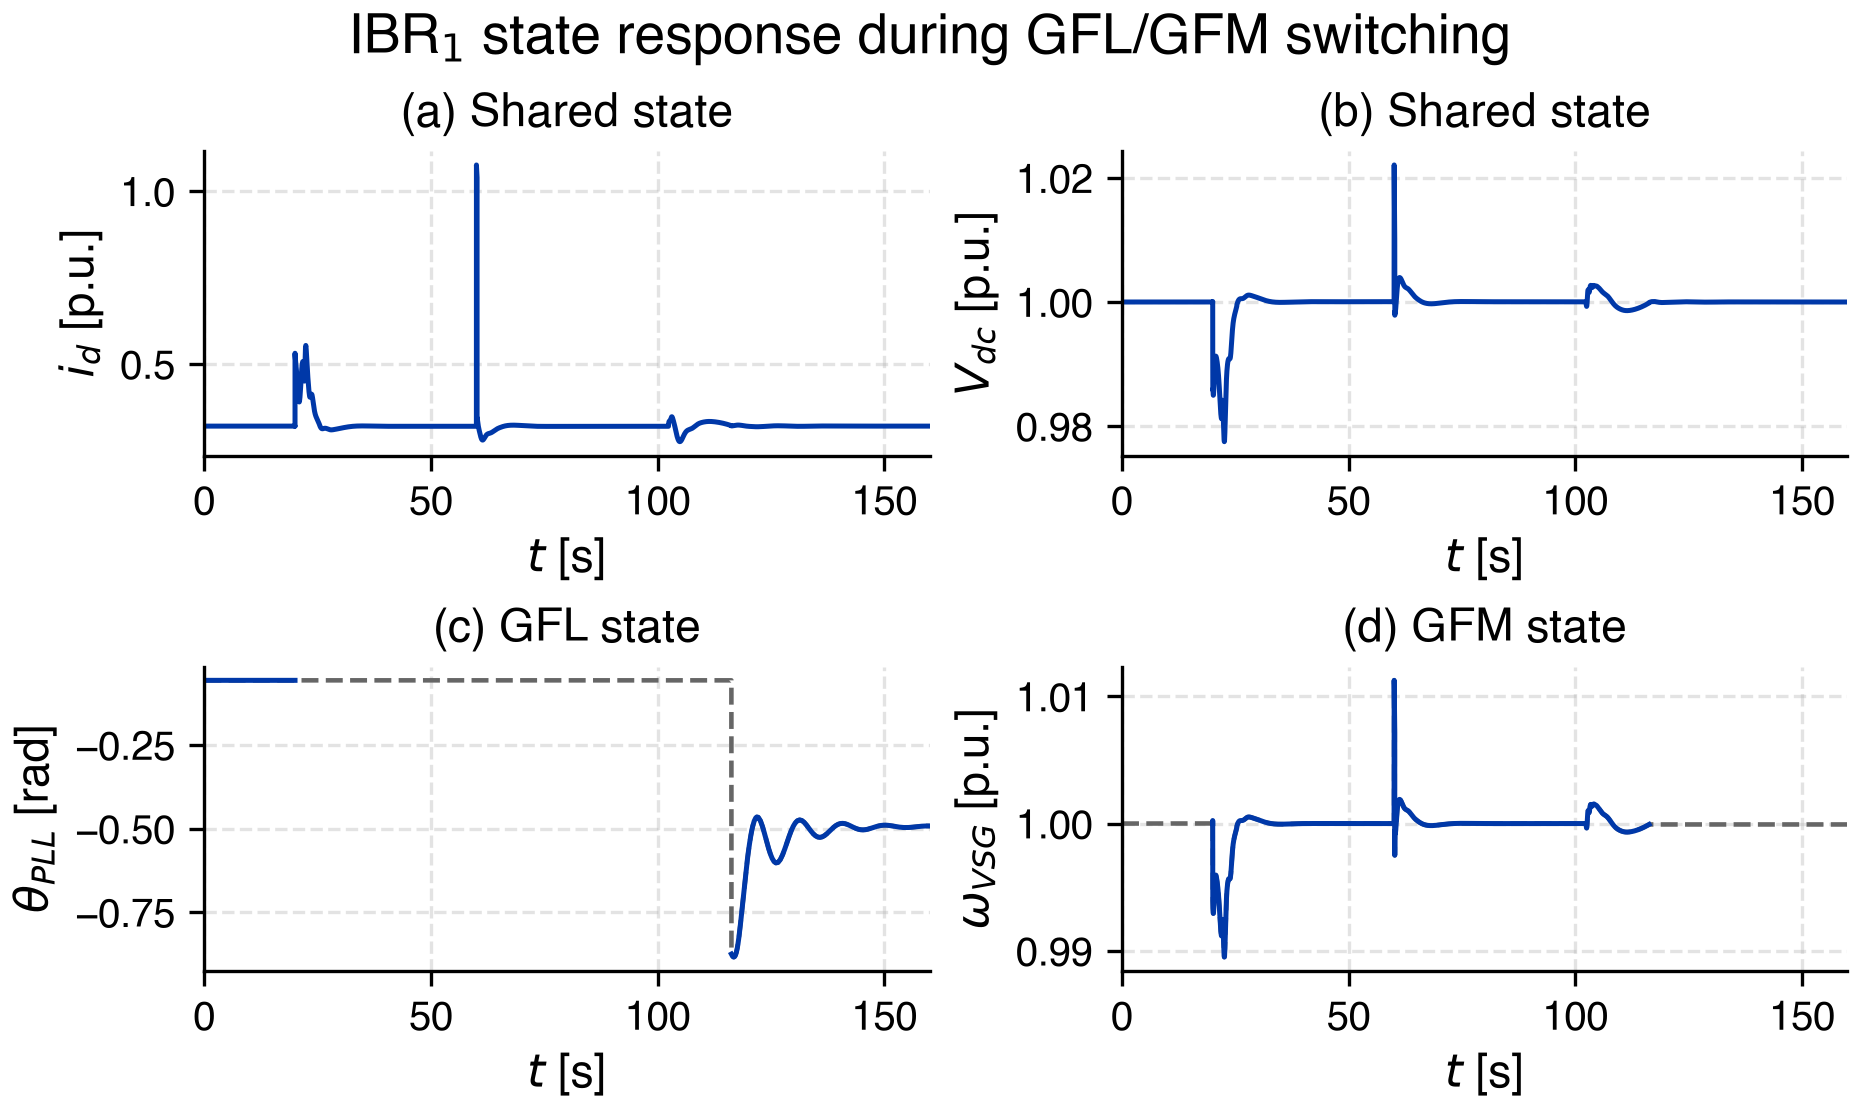
\includegraphics[width=\linewidth,height=5.45cm,keepaspectratio]{figures/ieee14_scenario_suite/sg_fault_cycle160_ibr_states_v15.png}\caption{IBR$_1$ states: $(a)$ $i_d,i_q$; $(b)$ $V_{dc},I_{dc}$; $(c)$ $\omega_{VSG}$; $(d)$ $E$}\end{figure}
{\scriptsize Blue = active; grey dashed = held stored state. IBR$_1$ only.\par}
\end{frame}
\begin{frame}{Result: Severity Index and Converter Mode}
\centering
\begin{figure}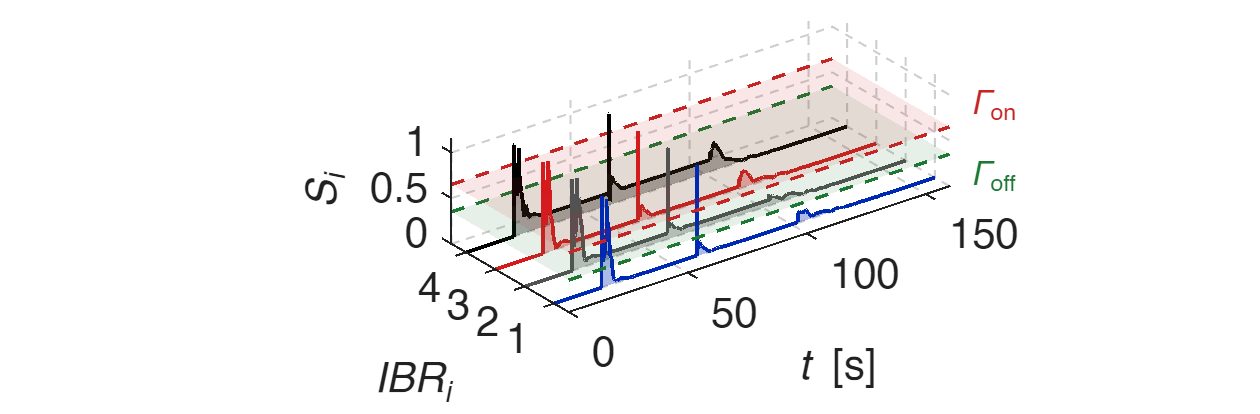
\includegraphics[width=.68\linewidth]{figures/ieee14_scenario_suite/sg_fault_cycle160_agsi3d.png}\caption{Severity index $S_i$ per converter.}\end{figure}

\vspace{1mm}
\begin{figure}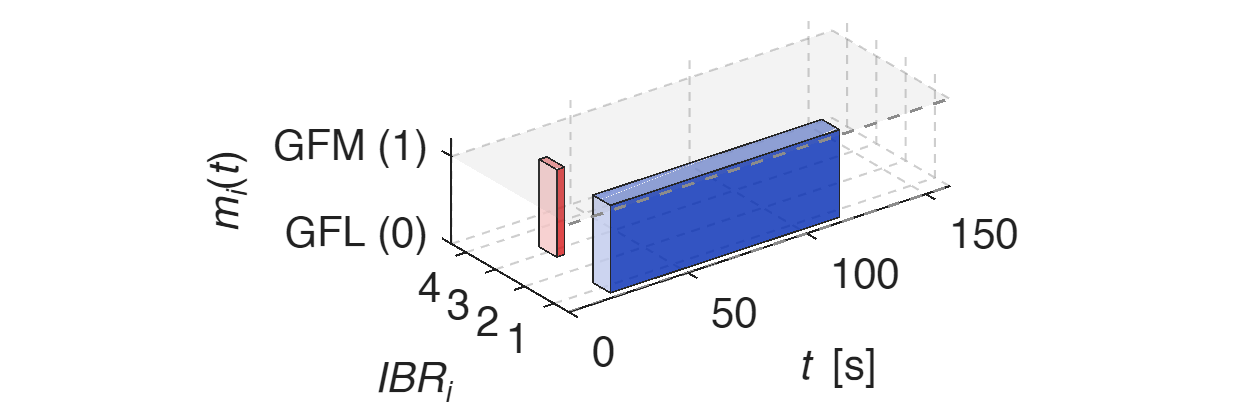
\includegraphics[width=.68\linewidth]{figures/ieee14_scenario_suite/sg_fault_cycle160_mode3d.png}\caption{Converter mode $m_i$ per converter: GFL = 0, GFM = 1.}\end{figure}
\end{frame}
\begin{frame}{Result: Voltage and Frequency}
\centering\begin{figure}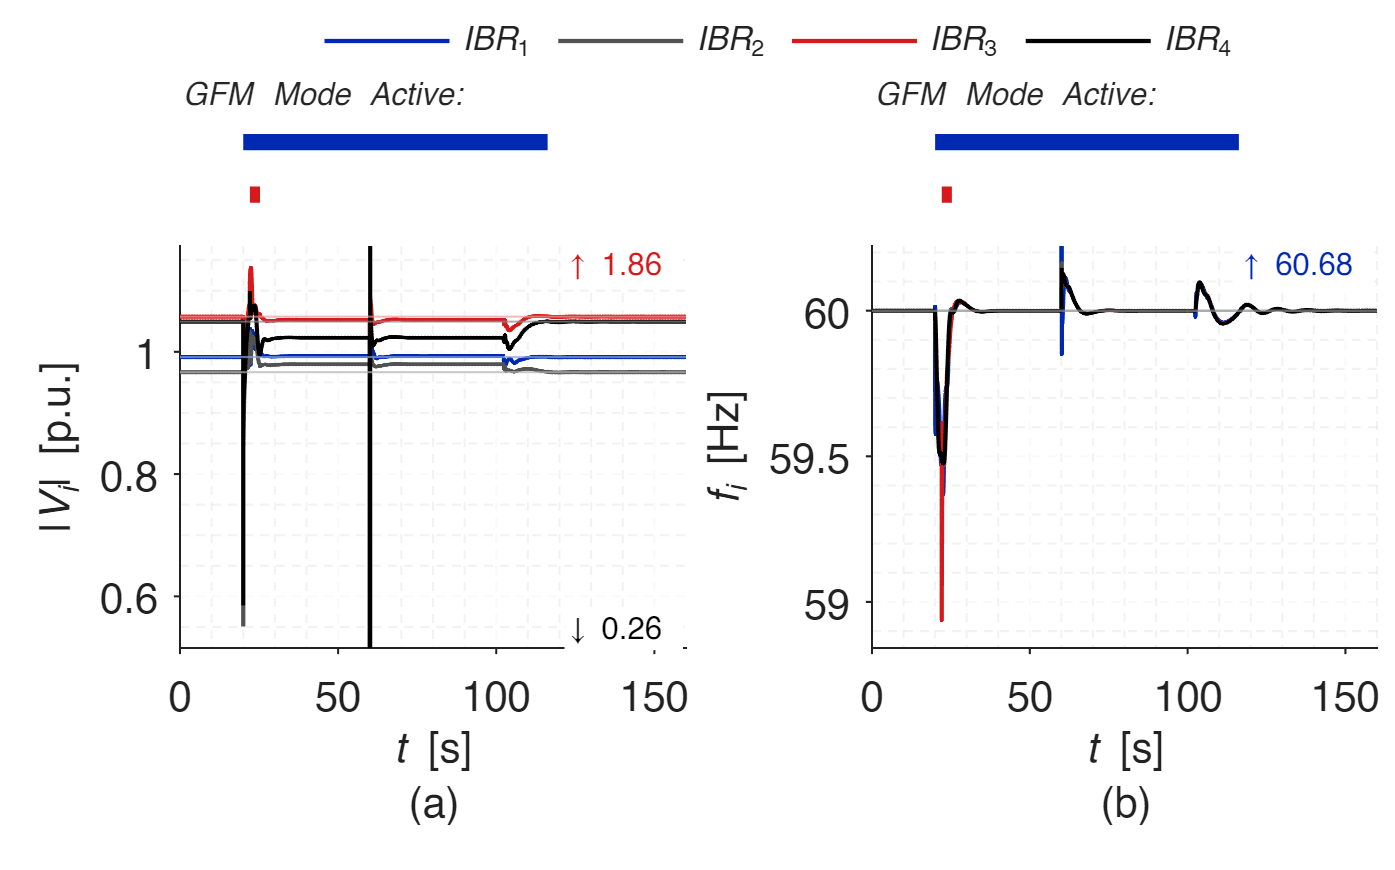
\includegraphics[width=\linewidth,height=5.9cm,keepaspectratio]{figures/ieee14_scenario_suite/sg_fault_cycle160_vf.png}\caption{Converter responses: $(a)$ bus-voltage magnitude and $(b)$ converter frequency.}\end{figure}
\end{frame}
\begin{frame}{Result: Active and Reactive Power}
\centering\begin{figure}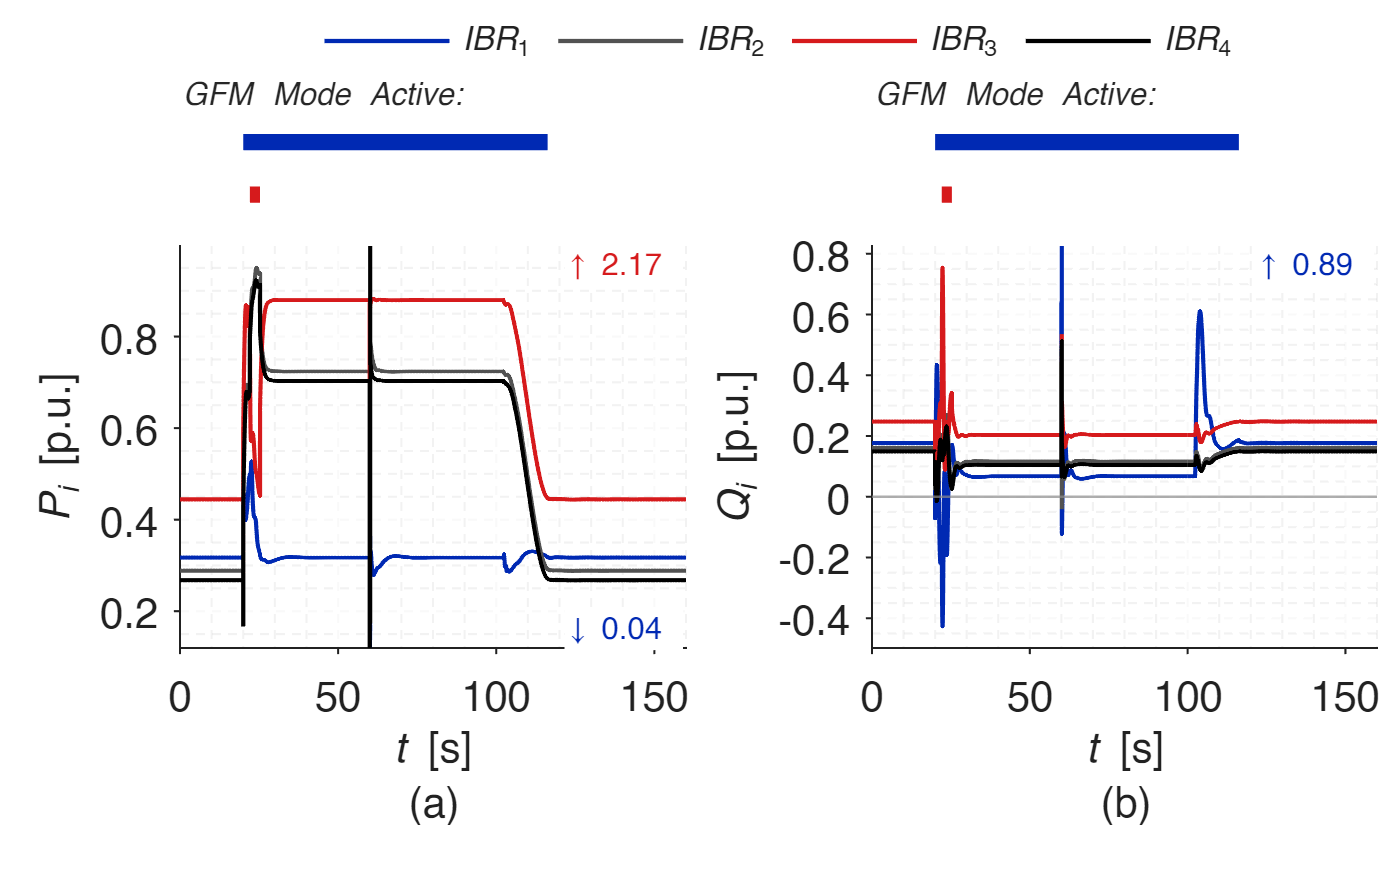
\includegraphics[width=\linewidth,height=5.9cm,keepaspectratio]{figures/ieee14_scenario_suite/sg_fault_cycle160_pq_mode.png}\caption{Converter power responses: $(a)$ active power and $(b)$ reactive power.}\end{figure}
\end{frame}
\begin{frame}{Fault Bus  Voltage and Frequency}
\centering\begin{figure}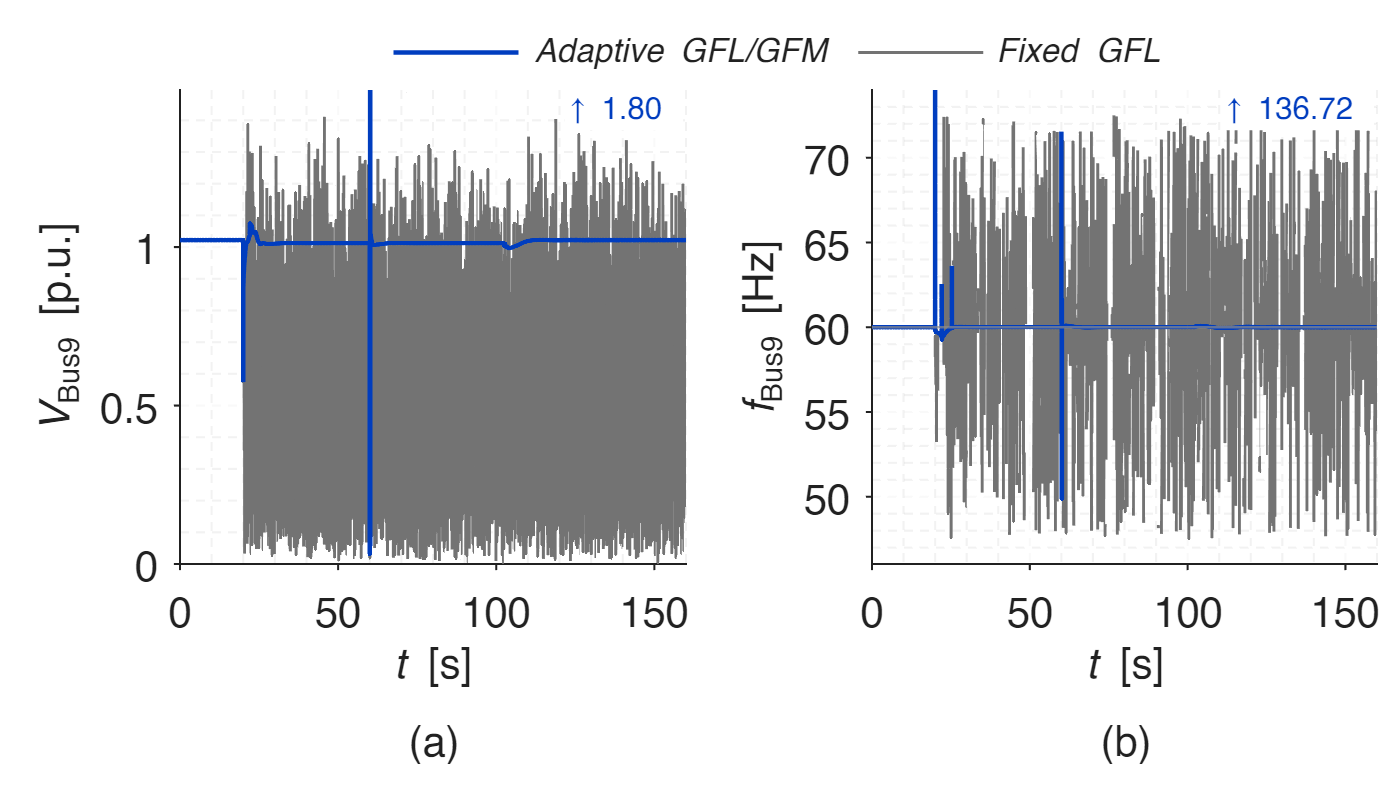
\includegraphics[width=\linewidth,height=5.75cm,keepaspectratio]{figures/ieee14_scenario_suite/sg_fault_cycle160_cmp_vf.png}\caption{Bus-9 responses for adaptive GFL/GFM and fixed-GFL cases: $(a)$ voltage magnitude and $(b)$ frequency.}\end{figure}
\end{frame}
\begin{frame}{Fault Bus Active and Reactive Power}
\centering\begin{figure}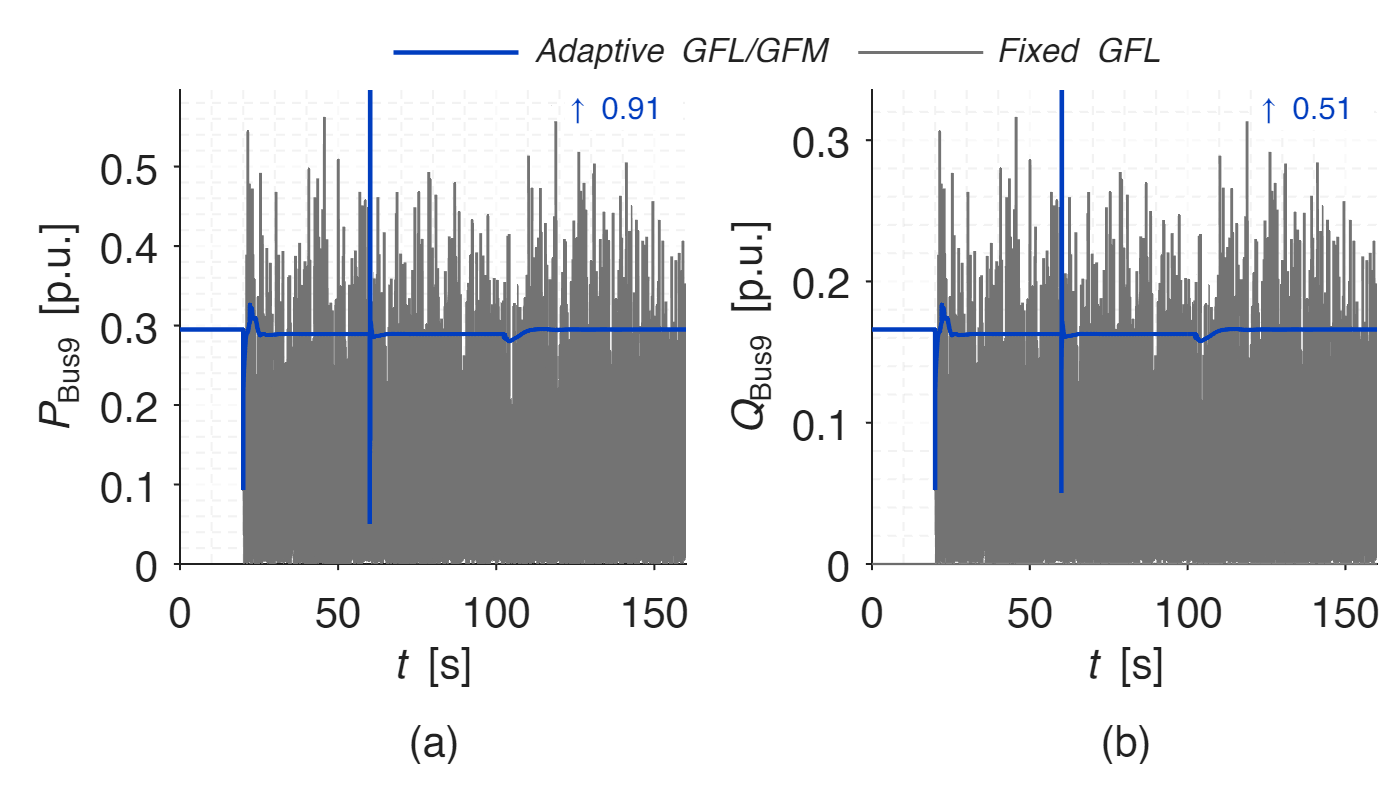
\includegraphics[width=\linewidth,height=5.75cm,keepaspectratio]{figures/ieee14_scenario_suite/sg_fault_cycle160_cmp_pq.png}\caption{Bus-9 power responses for adaptive GFL/GFM and fixed-GFL cases: $(a)$ active power and $(b)$ reactive power.}\end{figure}
\end{frame}

\section{Summary}
\begin{frame}{Summary}
\begin{columns}[t,onlytextwidth]
\column{.49\textwidth}\small
\textbf{Completed Development}\vspace{.15cm}
\begin{itemize}\setlength{\itemsep}{.35cm}
\item[\ckbox] Power flow and time-domain simulation.
\item[\ckbox] Switchable GFL/GFM converter model.
\item[\ckbox] Continuous physical and DC states during mode transfer.
\item[\ckbox] Adaptive switching based on voltage and frequency deviations.
\end{itemize}
\column{.46\textwidth}\small
\textbf{Future Development}\vspace{.15cm}
\begin{itemize}\setlength{\itemsep}{.45cm}
\item[\opbox] Establish admissible switching and dwell-time conditions for the hybrid DAE.
\item[\opbox] Simulation on larger-scale power systems.
\item[\opbox] Development of Intelligent switching control to manage transients and reduce switching errors
\end{itemize}
\end{columns}
\end{frame}

\section{References}
\begin{frame}{References}
\scriptsize
\begin{enumerate}\setlength{\itemsep}{.12cm}
\item N. Pogaku, M. Prodanovi\'{c}, and T. C. Green, ``Modeling, analysis and testing of autonomous operation of an inverter-based microgrid,'' \emph{IEEE Trans. Power Electronics}, 22(2), 613--625, 2007.
\item H. Ding, R. Kar, Z. Miao, and L. Fan, ``A novel design for switchable grid-following and grid-forming control,'' \emph{IEEE Trans. Sustainable Energy}, 16(2), 1301--1314, 2025.
\item MATPOWER, \emph{case14: IEEE 14-bus test case}, converted from the IEEE Common Data Format.
\item S. K. M. Kodsi and C. A. Ca\~nizares, \emph{Modeling and simulation of IEEE 14 bus system with FACTS controllers}, University of Waterloo, Technical Report 2003-3, 2003.
\item A. Yazdani and R. Iravani, \emph{Voltage-Sourced Converters in Power Systems}, Wiley/IEEE Press, 2010.
\item R. Teodorescu, M. Liserre, and P. Rodr\'{i}guez, \emph{Grid Converters for Photovoltaic and Wind Power Systems}, Wiley/IEEE Press, 2011.
\item K. Sakimoto, Y. Miura, and T. Ise, ``Virtual synchronous generator without phase locked loop based on current controlled inverter and its parameter design,'' \emph{IEEJ Trans. Power and Energy}, 135(7), 462--470, 2015.
\end{enumerate}
\end{frame}
\end{document}
